% !TeX root = Informe_Lab8.tex
% !TeX root = Informe_Lab8.tex
\documentclass[journal]{IEEEtran}
%
\usepackage{instructivo}  
\graphicspath{{./}{./fig/}}

\usepackage{circuitikz}
\usepackage{float}
\usepackage{graphicx}
\usepackage[skip=5pt]{caption}
\usepackage{flafter}
\usepackage{needspace}
\usepackage{csquotes}
\usepackage{upgreek}


\hyphenation{op-tical net-works semi-conduc-tor}

\renewcommand\IEEEkeywordsname{Palabras clave}

\begin{document}
\title{Respuesta en frecuencia de un amplificador BJT}


\author{Juan~P.~Elizondo~Espinoza,~\IEEEmembership{Estudiante,~TEC}
        y~Matías~A.~Camacho~Abarca,~\IEEEmembership{Estudiante,~TEC.}
}


\markboth{TEC.~EL-3215 Laboratorio de Electrónica Analógica, IS~2025}%
{EL3215 Laboratorio de Electrónica Analógica}


\maketitle


\begin{abstract}
Este experimento pretendió analizar el comportamiento de dos topologías ya conocidas en amplificadores de señales; pero esta vez haciendo uso de
transistores de efecto de campo (JFETs). Para llevarlo a cabo, se contruyeron tres circuitos diferentes, el primero con una topología de 
fuente común, el segundo con una topología de drenador común y el tercero presenta una modificación que consiste en agregar una fuente de corriente.
Logrando así, analizar el comportamiento de las señales en CD y CA para cada uno de los circuitos. 
Este experimento pretendió analizar el comportamiento de dos topologías ya conocidas en amplificadores de señales; pero esta vez haciendo uso de
transistores de efecto de campo (JFETs). Para llevarlo a cabo, se contruyeron tres circuitos diferentes, el primero con una topología de 
fuente común, el segundo con una topología de drenador común y el tercero presenta una modificación que consiste en agregar una fuente de corriente.
Logrando así, analizar el comportamiento de las señales en CD y CA para cada uno de los circuitos. 
\end{abstract}

\begin{IEEEkeywords}
JFETs, polarización, ganancia, tensión, corriente.
\end{IEEEkeywords}


%%%%%%%%%%%%%%%%%%%%%%%%%%%%%%%%%%%%%%%%%%%%%%%%%%%%%%%%%%%%%%%%%%%%%%%%%%%%%%%%%%%%%%%%%%%%%%
%%%%%%%%%%%%%%%%%%%%%%%%%%%%%%%%%%%%%%%%%%%%%%%%%%%%%%%%%%%%%%%%%%%%%%%%%%%%%%%%%%%%%%%%%%%%%%
\section{Introducción}

\IEEEPARstart{E}l transistor de efecto de campo, también conocido como JFET, trabaja con una unión PN
polarizada de manera inversa (con tensiones negativas). Cuando se le aplica un voltaje $V_{\text{DD}}$, se genera 
una tensión entre el drenaje y la fuente, lo cual induce corriente desde el drenaje hasta la fuente. La forma en la 
que se controla la cantidad corriente $I_{\text{D}}$ en el transistor, consiste en variar la resistencia del transistor
al variar el ancho del canal, el cual se modifica debido a la región de empobrecimiento a lo largo de la unión PN;
dicha región de empobecimiento, aparece al polarizar en inversa las uniones compuerta y fuente ($V_{\text{GS}}$)~\cite{Floyd}.

Cabe aclarar, que en un JFET la corriente de drenaje $I_{\text{D}}$ va disminuyendo conforme la tension $V_{\text{GS}}$ se
hace cada vez más negativa, pues con esto se ensancha la región de empobrecimiento, hasta que se llega a la tensión 
de corte en donde el canal se cierra por completo.

Con este tipo de transistores, también se pueden construir amplificadores con topologías fuente común y 
drenador común, bajo una idea muy similar a como se trabaja con transistores MOSFET y BJT. Esto es lo que se pretendió 
aplicar en el laboratorio; para el caso de los amplificadores de fuente común, la señal de entrada se aplica en la compuerta
y la salida es tomada directamente desde el drenador del transistor; en el caso de la topología drenador común, lo que cambia
es que ahora la salida será tomada desde la fuente del transistor~\cite{Floyd}.
\IEEEPARstart{E}l transistor de efecto de campo, también conocido como JFET, trabaja con una unión PN
polarizada de manera inversa (con tensiones negativas). Cuando se le aplica un voltaje $V_{\text{DD}}$, se genera 
una tensión entre el drenaje y la fuente, lo cual induce corriente desde el drenaje hasta la fuente. La forma en la 
que se controla la cantidad corriente $I_{\text{D}}$ en el transistor, consiste en variar la resistencia del transistor
al variar el ancho del canal, el cual se modifica debido a la región de empobrecimiento a lo largo de la unión PN;
dicha región de empobecimiento, aparece al polarizar en inversa las uniones compuerta y fuente ($V_{\text{GS}}$)~\cite{Floyd}.

Cabe aclarar, que en un JFET la corriente de drenaje $I_{\text{D}}$ va disminuyendo conforme la tension $V_{\text{GS}}$ se
hace cada vez más negativa, pues con esto se ensancha la región de empobrecimiento, hasta que se llega a la tensión 
de corte en donde el canal se cierra por completo.

Con este tipo de transistores, también se pueden construir amplificadores con topologías fuente común y 
drenador común, bajo una idea muy similar a como se trabaja con transistores MOSFET y BJT. Esto es lo que se pretendió 
aplicar en el laboratorio; para el caso de los amplificadores de fuente común, la señal de entrada se aplica en la compuerta
y la salida es tomada directamente desde el drenador del transistor; en el caso de la topología drenador común, lo que cambia
es que ahora la salida será tomada desde la fuente del transistor~\cite{Floyd}.

%%%%%%%%%%%%%%%%%%%%%%%%%%%%%%%%%%%%%%%%%%%%%%%%%%%%%%%%%%%%%%%%%%%%%%%%%%%%%%%%%%%%%%%%%%%%%%
%%%%%%%%%%%%%%%%%%%%%%%%%%%%%%%%%%%%%%%%%%%%%%%%%%%%%%%%%%%%%%%%%%%%%%%%%%%%%%%%%%%%%%%%%%%%%%
\section{Cirtuitos de mediciones}
Se presenta a continuación los circuitos construidos para la elaboración de este laboratorio. Se montaron 2 circuitos de tal manera que el circuito 1 sirvió para estudiar la respuesta en bajas frecuencias y el circuito 2 para estudiar la respuesta en altas frecuencias. Los transistores utilizados fueron BJTs 2N3904.
Se midieron los parámetros de polarización en corriente directa y parámetros en corriente alterna.


\subsection{Circuitos de Medición}

\begin{figure}[H]
        \centering
        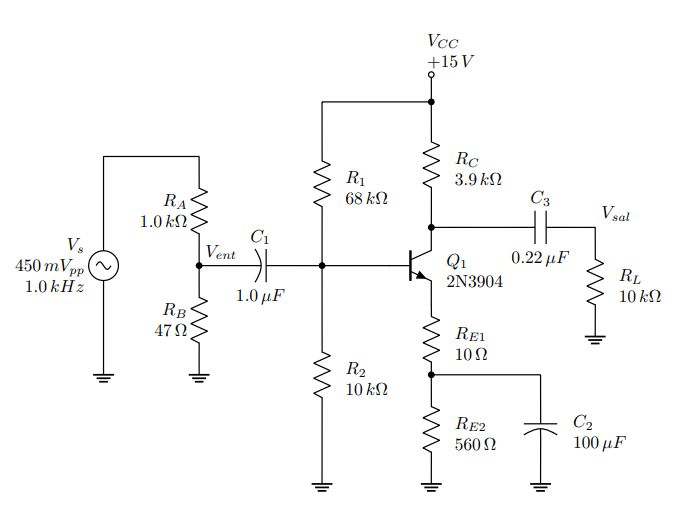
\includegraphics[width=3.4in]{Circuito1.png}
        \caption{Circuito 1}
        \label{fig:SignalExperimental_024}
\end{figure}

\begin{figure}[H]
        \centering
        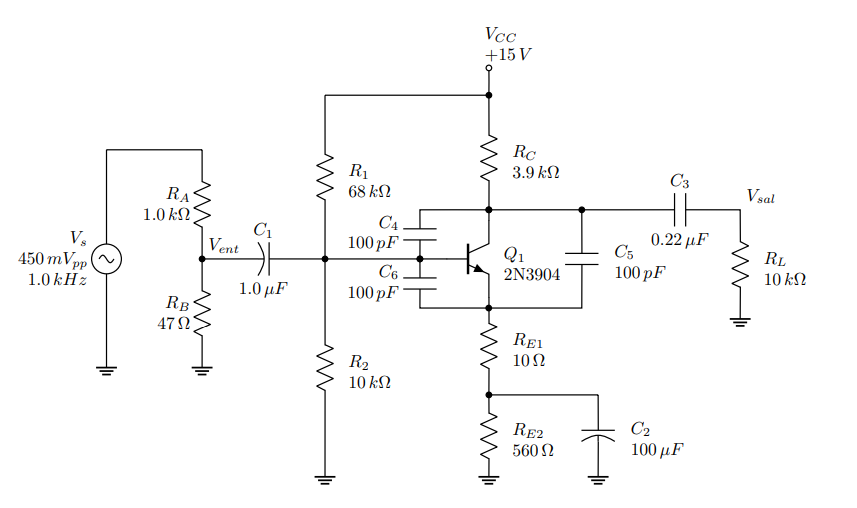
\includegraphics[width=3.4in]{Circuito2.png}
        \caption{Circuito 2}
        \label{fig:SignalExperimental_044}
\end{figure}

\vspace{1cm}


\subsection{Resultados}


\begin{table}[H]
        \centering
        \renewcommand{\arraystretch}{1.5}
        \caption{Valores de resistencias utilizadas en los circuitos 1 y 2}
        \begin{tabular}{ >{\centering\arraybackslash}m{2.5cm} >{\centering\arraybackslash}m{2.5cm} >{\centering\arraybackslash}m{2.5cm} }
                \hline
            \centering
            Componente & Valor requerido & Valor medido\\ 
            \hline
            \centering
            $R_A$ ($\mathrm{k}\Omega$) & $1$  & $1.000~58$  \\ 
            $R_B$ ($\Omega$) & $47$  & $49.907~6$  \\
            $R_C$ ($\mathrm{k}\Omega$) & $3.9$  & $3.855~47$  \\
            $R_1$ ($\mathrm{k}\Omega$) & $68$  & $67.771~6$ \\
            $R_2$ ($\mathrm{k}\Omega$) & $10$  & $9.925~77$ \\
            $R_L$ ($\mathrm{k}\Omega$) & $10$  & $9.937~73$ \\
            $R_{E1}$ ($\Omega$) & $10$  & $10.0248$ \\
            $R_{E2}$ ($\Omega$) & $560$  & $555.329$ \\
            \hline
        \end{tabular}
        \label{tabla1}
    \end{table}
    
\begin{table}[H]
        \centering
        \renewcommand{\arraystretch}{1.5}
        \caption{Valores de capacitores utilizados en el circuito 1}
        \begin{tabular}{ >{\centering\arraybackslash}m{2.5cm} >{\centering\arraybackslash}m{2.5cm} >{\centering\arraybackslash}m{2.5cm} }
                \hline
            Componente & Valor requerido ($\upmu\mathrm{F}$) & Valor medido ($\upmu\mathrm{F}$)\\ 
            \hline
            \centering
            $C_1$ & $1$  & $1.038~3$  \\ 
            $C_2$ & $100$  & $94$ \\
            $C_3$ & $0.22$  & $0.258~6$ \\
            \hline
        \end{tabular}
        \label{tabla2}
    \end{table}    

\begin{table}[H]
        \centering
        \renewcommand{\arraystretch}{1.5}
        \caption{Valores de capacitores utilizados en el circuito 2}
        \begin{tabular}{ >{\centering\arraybackslash}m{2.5cm} >{\centering\arraybackslash}m{2.5cm} >{\centering\arraybackslash}m{2.5cm} }
                \hline
            Componente & Valor requerido & Valor medido\\ 
            \hline
            \centering
            $C_1$ ($\upmu\mathrm{F}$) & $1$  & $1.038~3$  \\ 
            $C_2$ ($\upmu\mathrm{F}$) & $100$  & $94$ \\
            $C_3$ ($\upmu\mathrm{F}$) & $0.22$  & $0.258~6$ \\
            $C_4$ ($\mathrm{p}$) & $100$ & $98.3$ \\
            $C_5$ ($\mathrm{p}$) & $100$ & $104.5$ \\
            $C_6$ ($\mathrm{p}$) & $100$ & $90.3$ \\
            \hline
        \end{tabular}
        \label{tabla3}
    \end{table}   

Para realizar el cálculo de las frecuencias críticas de corte inferior del circuito 1, se procedió a aislar los capacitores de los efectos de los otros capacitores. Por ejemplo, se colocó un capacitor de $1000~\upmu\mathrm{F}$ en paralelo de C\textsubscript{2} y otro sobre C\textsubscript{3}; esto causó que la respuesta en frecuencia de estos capacitores tenga muy poco efecto sobre la salida del amplificador.
La señal de salida en banda media se ajustó a alrededor de $10~\mathrm{kHz}$ y se ajustó la
señal para ser observada hasta una caída en la ganancia de $3~\mathrm{dB}$. La frecuencia a la que se dio esa reducción representó la frecuencia crítica inferior debido al capacitor C\textsubscript{1}. El mismo procedimiento
se realizó para C\textsubscript{2} y C\textsubscript{3}.

\begin{table}[H]
        \centering
        \renewcommand{\arraystretch}{1.5}
        \caption{Frecuencias críticas de corte inferior, circuito 1}
        \begin{tabular}{ >{\centering\arraybackslash}m{2.5cm} >{\centering\arraybackslash}m{2.5cm} >{\centering\arraybackslash}m{2.5cm} }
                \hline
            Capacitor & Valor requerido ($\mathrm{Hz}$) & Valor medido ($\mathrm{Hz}$)\\ 
            \hline
            \centering
            $C_1$ & $51.303~8$  & $54.118$  \\ 
            $C_2$ & $69.812~4$  & $68.942$ \\
            $C_3$ & $52.045~4$  & $45.983$ \\
            $\mathrm{General}$ & $173.161~6$  & $125.83$ \\
            \hline
        \end{tabular}
        \label{tabla4}
    \end{table}    

También se calculó el valor de la frecuencia crítica inferior de C\textsubscript{2} si el valor de C\textsubscript{2} fuera modificado a aproximadamente $35.5~\upmu\mathrm{F}$ para conseguir una frecuencia de corte
general de $300~\mathrm{Hz}$.

\begin{table}[H]
        \centering
        \renewcommand{\arraystretch}{1.5}
        \caption{Frecuencias críticas de corte inferior de $C_2$, bsucando que la frecuencia crítica general inferior sea de $\mathrm{300~Hz}$}
        \begin{tabular}{ >{\centering\arraybackslash}m{2.5cm} >{\centering\arraybackslash}m{2.5cm} >{\centering\arraybackslash}m{2.5cm} }
                \hline
            Valor calculado de $C_2$ & Valor teórico ($\mathrm{Hz}$) & Valor medido ($\mathrm{Hz}$)\\ 
            \hline
            \centering
            $C_2$ & $196.650~8$  & $209.899$  \\ 
            \hline
        \end{tabular}
        \label{tabla11}
    \end{table}  
Es importante que debido al bajo valor de V\textsubscript{ent}, se estimó este como $10~mV$ para ambos circuitos. 
\begin{table}[H]
        \renewcommand{\arraystretch}{1.5}
        \caption{Mediciones del circuito 1}
        \centering
        \begin{tabular}{ >{\centering\arraybackslash}m{2.5cm} >{\centering\arraybackslash}m{2.5cm} >{\centering\arraybackslash}m{2.5cm} }
                \hline
            Parámetro & Valor teórico & Valor medido\\ 
            \hline
            $V_B$ ($\mathrm{V}$) & $1.77$  & $1.816~82$  \\ 
            $V_E$ ($\mathrm{V}$) & $1.09$  & $1.157~29$  \\
            $V_C$ ($\mathrm{V}$) & $7.59$  & $7.164~76$  \\
            $V_{CE}$ ($\mathrm{V}$) & $6.50$  & $6.007~47$  \\
            $I_E$ ($\mathrm{mA}$) & $1.92$  & $2.047$ \\ 
            $|A_v|$  & $109.443$ & $115.5$  \\
            $V_{sal}$ & $1.057$  & $1.155$ \\
            \hline
        \end{tabular}
        \label{tabla5}
    \end{table}

\begin{figure}[H]
        \centering
        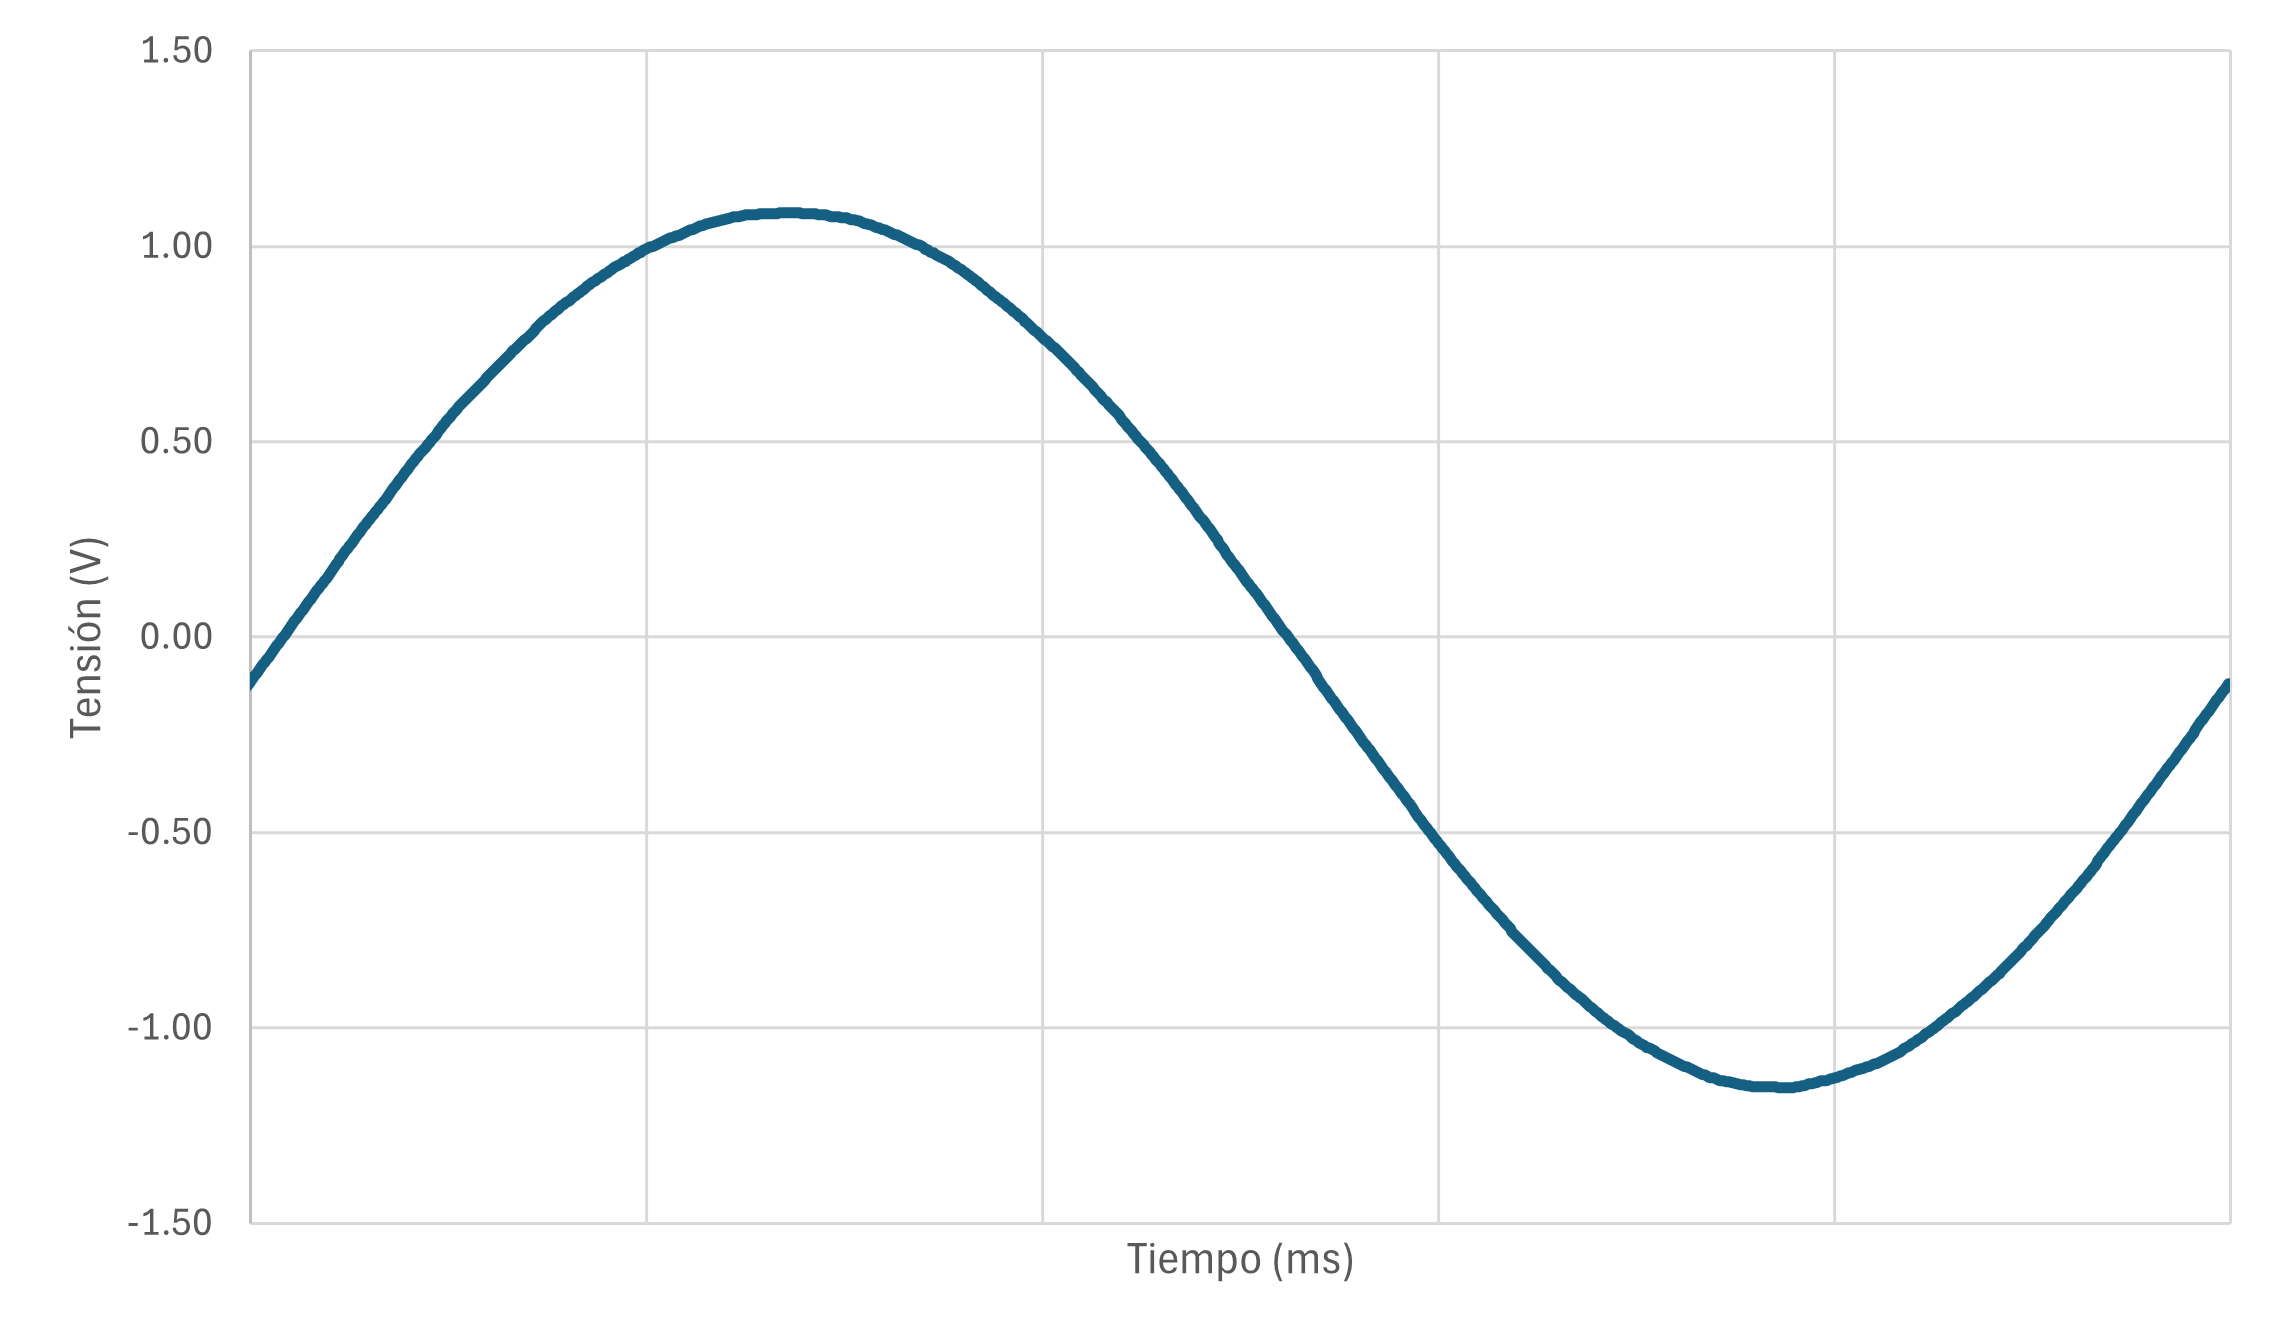
\includegraphics[width=3.4in]{OutC1.png}
        \caption{$V_{sal}$ obtenido experimentalmente en el circuito 1 durante un periodo}
        \label{fig:SignalExperimental_0222}
\end{figure}
    
\begin{table}[H]
        \renewcommand{\arraystretch}{1.5}
        \caption{Mediciones del circuito 2}
        \centering
        \begin{tabular}{ >{\centering\arraybackslash}m{2.5cm} >{\centering\arraybackslash}m{2.5cm} >{\centering\arraybackslash}m{2.5cm} }
                \hline
            Parámetro & Valor teórico & Valor medido\\ 
            \hline
            $V_B$ ($\mathrm{V}$) & $1.811~16$  & $1.806~24$  \\ 
            $V_E$ ($\mathrm{V}$) & $1.129~35$  & $1.156~78$  \\
            $V_C$ ($\mathrm{V}$) & $7.322~96$  & $7.392~27$  \\
            $V_{CE}$ ($\mathrm{V}$) & $6.193~61$  & $6.235~49$  \\
            $I_E$ ($\mathrm{mA}$) & $1.981~31$  & $2.046$ \\ 
            $|A_v|$  & $111.5449$ & $113.5$  \\
            $V_{sal}$ & $1.175~07$  & $1.135$ \\
            \hline
        \end{tabular}
        \label{tabla6}
    \end{table}

\begin{figure}[H]
        \centering
        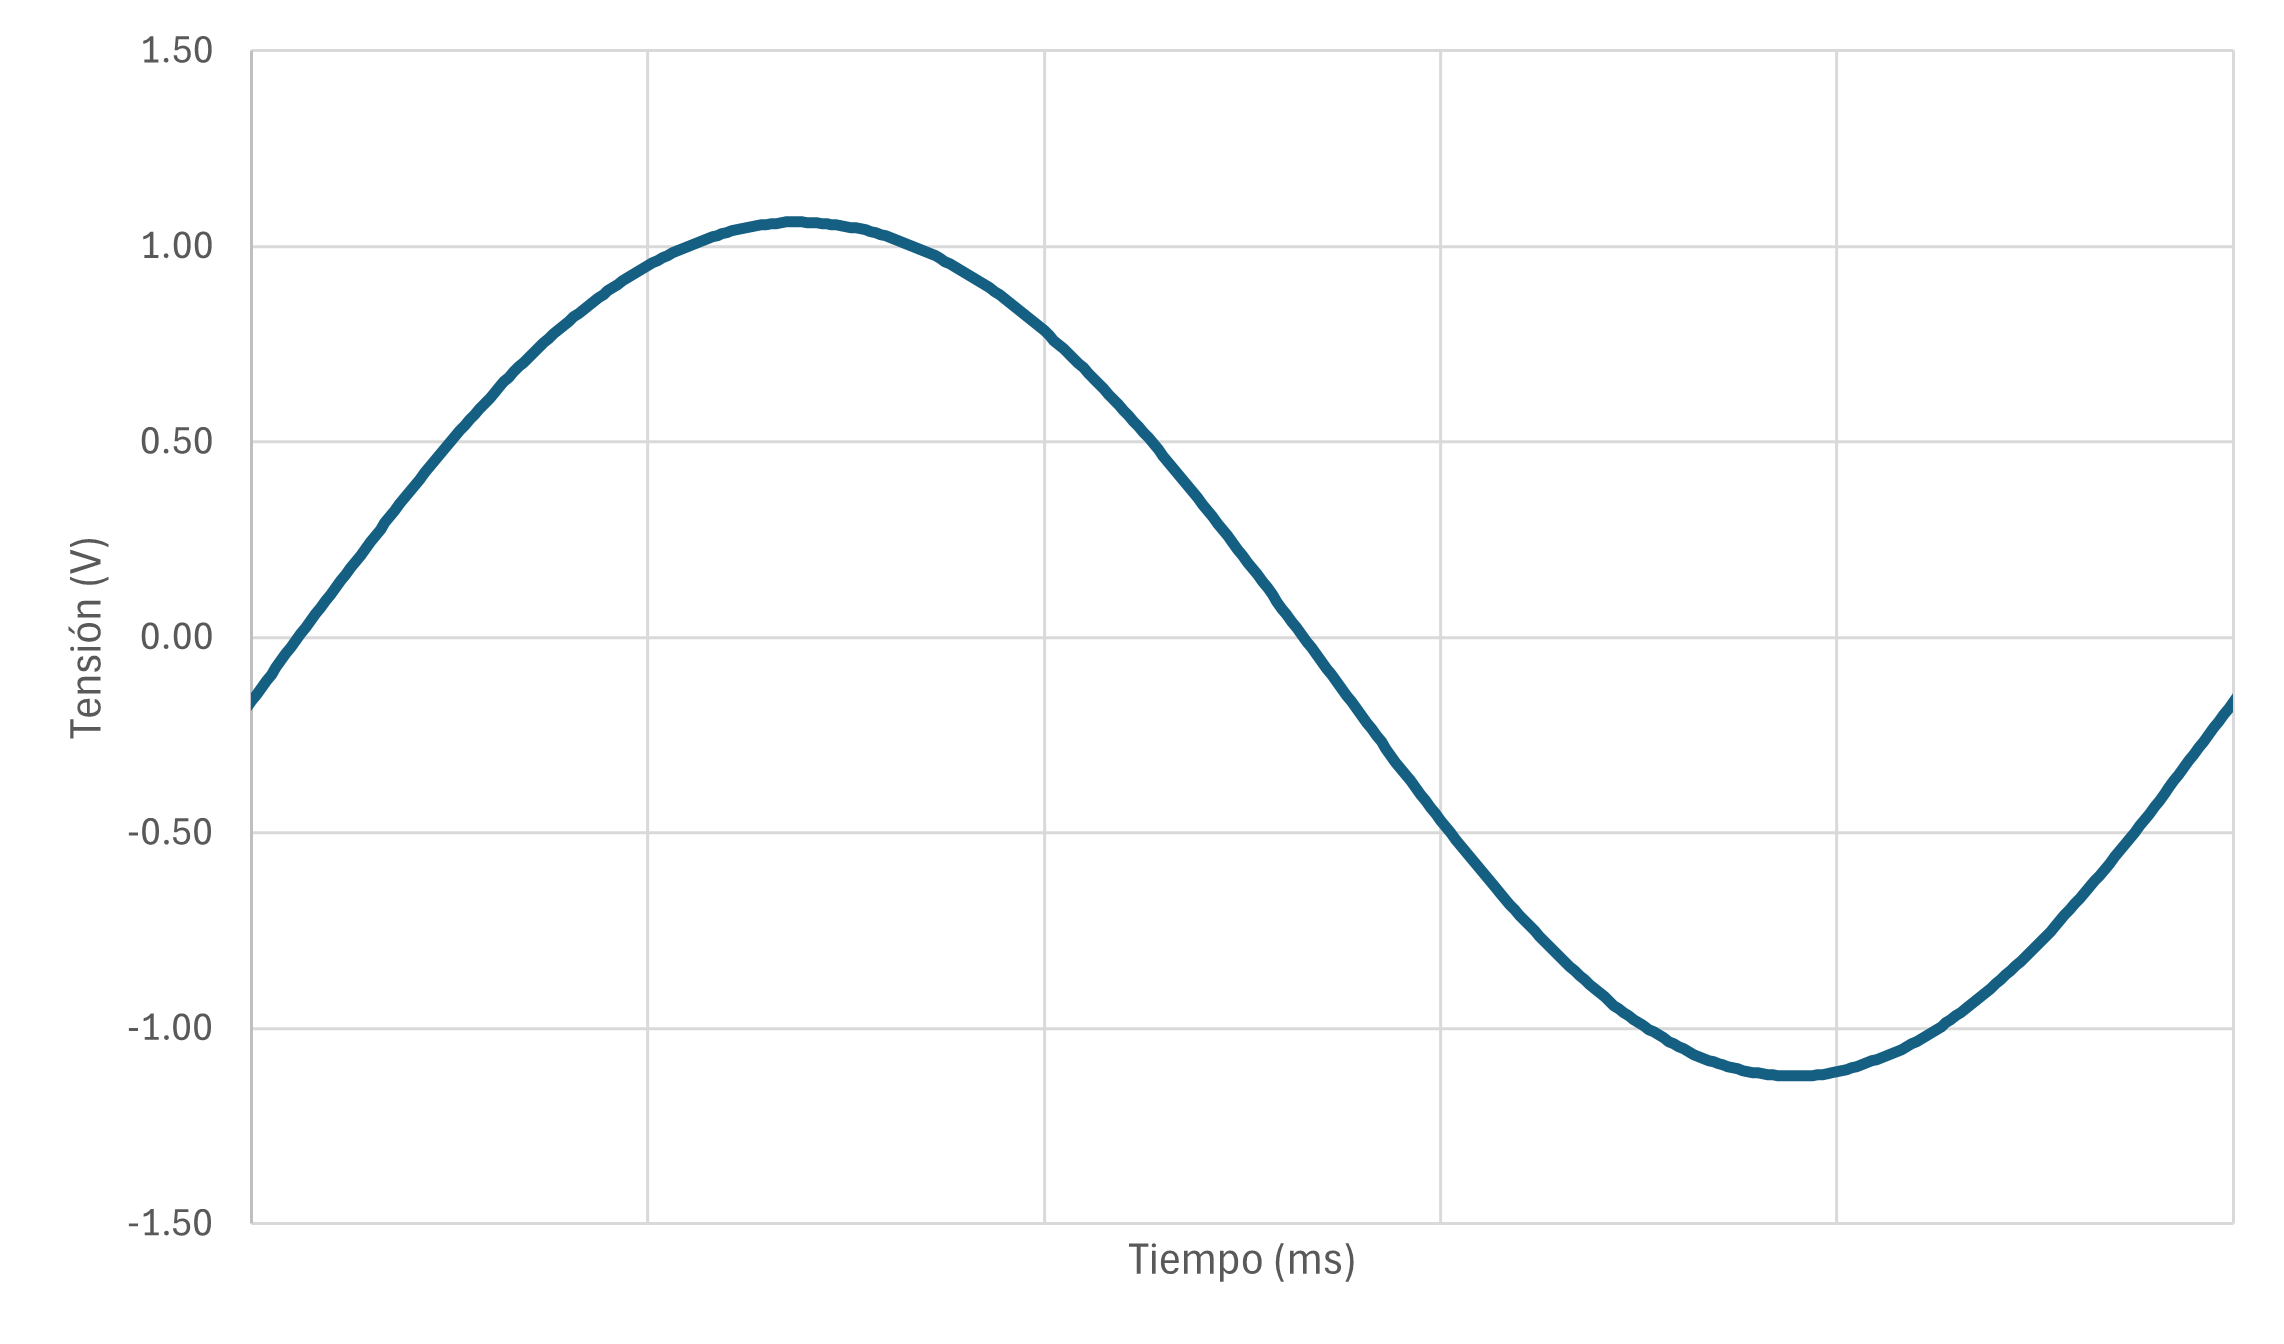
\includegraphics[width=3.4in]{OutC2.png}
        \caption{$V_{sal}$ obtenido experimentalmente en el circuito 2 durante un periodo}
        \label{fig:SignalExperimental_02}
\end{figure}

Para el cálculo de la frecuencia crítica superior general, se modificó la frecuencia de la fuente hasta observar una caida de $3~\mathrm{dB}$.

\begin{table}[H]
        \centering
        \renewcommand{\arraystretch}{1.5}
        \caption{Frecuencias crítica superior general, circuito 2}
        \begin{tabular}{ >{\centering\arraybackslash}m{2.5cm} >{\centering\arraybackslash}m{2.5cm} >{\centering\arraybackslash}m{2.5cm} }
                \hline
            Frecuencia & Valor requerido ($\mathrm{kHz}$) & Valor medido ($\mathrm{kHz}$)\\ 
            \hline
            \centering
            $f_{cu}$ & $166.331$  & $165.80$  \\ 
            \hline
        \end{tabular}
        \label{tabla7}
    \end{table}   

\subsection{Análisis de Resultados}
Con la intención de lograr los mejores resultados posibles, se trató de ajustar los 
valores reales de los componentes a utilizar, de forma que coincidieran lo más cerca con
los valores teóricos necesarios, aunque siempre existen ciertas discrepancias.

Para el primer circuito, se observan ciertas diferencias algo significativas entre los valores
recolectados, con respecto a lo esperado teóricamente; esto en cuanto a parámetros de polarización. 
Si se observan las señales de entrada y salida en este primer circuito, se puede notar una leve diferencia
en la señal de salida respecto a lo esperado (es menor al valor teórico); además, en el semiciclo negativo
existe un recorte en la onda, que provoca una alteración en la ganancia durante ese tiempo, esto se intentó 
solucionar durante la práctica de laboratorio; no obstante, se debía de bajar considerablemente la señal de entrada.

Para el caso de la topología de drenador común, la amplitud de la señal de salida es de un valor muy cercano al teórico, 
su fase es correcta y en este caso, no presenta recortes extraños que alteren la ganancia. 

Por último, el tercer circuito (modificado con una fuente de corriente), es el que presenta menos margen de error
en cuanto a la diferencia entre valores experimentales y valores teóricos. La señal de salida es prácticamente
igual a la esperada, incluso en este caso, presenta un desfase de cero grados tal cual debe ser. 

\section{Conclusiones}
Fue posible obtener los valores teóricos de polarización en CD y los parámetros en CA para la topología de fuente
común con JFETs, comprobando así que la señal de salida en esta topología, presenta un desfase cercano a los $180^\circ$
con respecto a la señal de entrada, igual a como ocurre con otros transistores.

Al igual que con la topología de drenador común, con fuente común se expusieron los parámetros de polarización en CD
y el análisis de los valores para las señales de CA. En esta configuración, no existe desfase significativo entre las 
señales de entrada y salida, según se esperaba. 
Fue posible obtener los valores teóricos de polarización en CD y los parámetros en CA para la topología de fuente
común con JFETs, comprobando así que la señal de salida en esta topología, presenta un desfase cercano a los $180^\circ$
con respecto a la señal de entrada, igual a como ocurre con otros transistores.

Al igual que con la topología de drenador común, con fuente común se expusieron los parámetros de polarización en CD
y el análisis de los valores para las señales de CA. En esta configuración, no existe desfase significativo entre las 
señales de entrada y salida, según se esperaba. 
\appendices

\section{}

\begin{IEEEbiographynophoto}{Matías A. Camacho Abarca}
        Estudiante del Instituto Tecnológico de Costa Rica en la carrerra de ingeniería en electrónica desde
        2023. Beneficiario de beca de excelencia académica por el Instituto Tecnológico de
        Costa Rica desde 2023. Como estudiante, sus
        intereses incluyen investigación y desarrollo.
        Correo electrónico: jeacamacho@estudiantec.cr
\end{IEEEbiographynophoto}

\begin{IEEEbiographynophoto}{Juan P. Elizondo Espinoza}
        Oriundo de Pérez Zeledón. Realizó sus estudios de secundaria en el SNCCCR, sede UNA Región Brunca, y actualmente cursa la carrera de Ingeniería Electrónica en el Instituto Tecnológico de Costa Rica (TEC). 
        
        Anteriormente, fue estudiante de la Universidad de Costa Rica (UCR) durante el año 2022 y participó en programas de estudio en matemática en la Universidad Nacional (UNA) durante los años 2020 y 2021. 
        
        Cuenta con preparación y/o experiencia en áreas como:
        \begin{itemize}
            \item Arquitectura básica de redes, certificado por CISCO CCNA V7 (ITN), (2021).
            \item Principios de ciberseguridad, certificado por CISCO Systems, (2022).
            \item Programa de tutorías estudiantiles, Tecnológico de Costa Rica, (2024).
        \end{itemize}
        
        Correo: juelizondo@estudiantec.cr
\end{IEEEbiographynophoto}

%%\bibliographystyle{IEEEtran}
%%\bibliography{literatura}

\begin{thebibliography}{11}
    \bibitem{Floyd}
    Thomas L. Floyd, \emph{Dispositivos Electrónicos}, 8ª edición, Pearson, 2008.
\end{thebibliography}
%%\bibliographystyle{IEEEtran}
%%\bibliography{literatura}

\end{document}